\documentclass[dvipdfmx,12pt]{beamer}

\usepackage{bxdpx-beamer}% dvipdfmxなので必要
\usepackage{pxjahyper}% 日本語で'しおり'したい
\usepackage{minijs}% min10ヤダ
\renewcommand{\kanjifamilydefault}{\gtdefault}% 既定をゴシック体に

\usetheme[option]{PaloAlto}
\usepackage{url}
\usepackage{hyperref}

\usepackage{amsmath}
\usepackage{amssymb}
\usepackage{amsfonts}
%\usepackage{euler} \usepackage{graphicx}
\usepackage{color}
\usepackage[cache=true]{minted}

\logo{{\large$\mathbb{N}$}}
\title[ヒューマンセンシング]{主専攻実験 最終報告会 \\ ヒューマンセンシング}
\author[荻野夏樹]{情報科学類 201611353 \\ 荻野夏樹}
\date{\today}
\begin{document}
\maketitle
\section{目的}
\subsection{使用したデータセット}
\begin{frame}
	\frametitle{使用したデータセット:CelebA}
	\begin{figure}[htbp]
	\begin{center}
	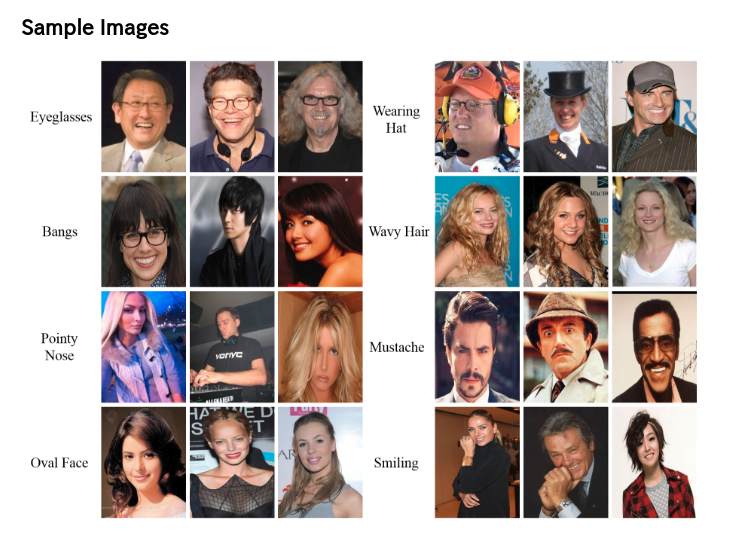
\includegraphics[width=0.7\hsize]{./SelebA_discription.png}
	\end{center}
	\end{figure}

	\begin{enumerate}
		\item 10,177人の異なる人物
		\item 202,599 枚の画像
		\item 5つ(目鼻口とか)の位置情報
		\item その他眼鏡など40属性
	\end{enumerate}
\end{frame}

\subsection{実験の目的}
\begin{frame}
	\frametitle{実験の目的}
	{\large GAN(敵対的生成ネットワーク)\\を用いて顔画像の生成モデルを推論し、\\精度(inception score)を高める}
	\begin{enumerate}
		\item Generator: 乱数から本物の画像に似せた画像を生成
		\item Discriminator: Gの出力と本物の画像を判別する
	\end{enumerate}
	対立する2つのNNを交互に学習することで、切磋琢磨してくれることを期待する
\end{frame}

\subsection{なぜGAN}
\begin{frame}
	\frametitle{なぜGANに興味を持ったか}
	\begin{figure}[htbp]
	\begin{center}
	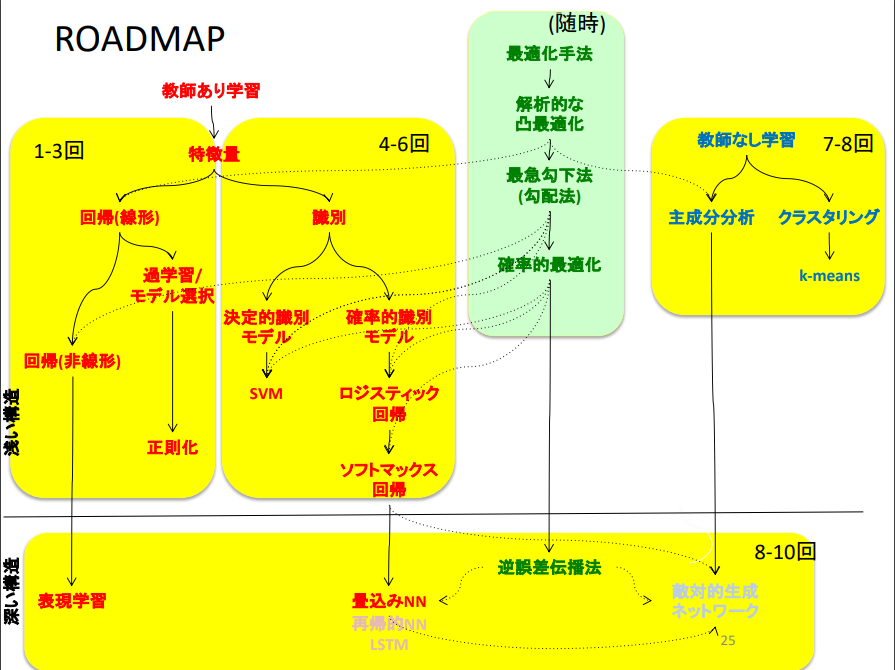
\includegraphics[width=0.7\hsize]{./road_map.png}
	\end{center}
	\end{figure}
	画像認識工学と機械学習
\end{frame}

\subsection{inception scoreとは}
\begin{frame}
	\frametitle{inception scoreとは}
	\begin{figure}[htbp]
	\begin{center}
	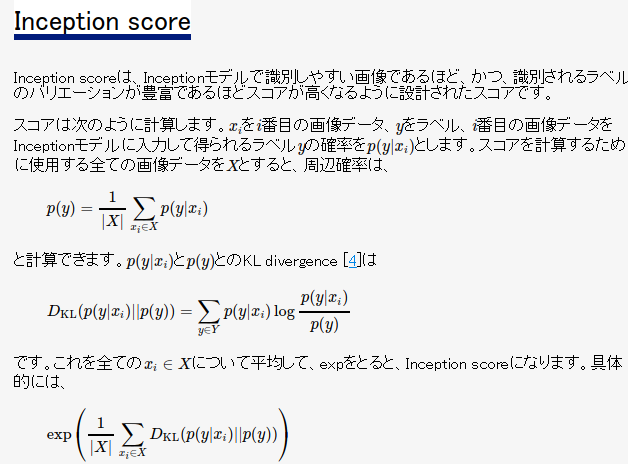
\includegraphics[width=\hsize]{./inception_score_discription.png}
	\end{center}
	\end{figure}
\end{frame}

\subsection{目的関数}
\begin{frame}
	\frametitle{目的関数とミニバッチ学習}
	\begin{figure}[htbp]
	\begin{center}
	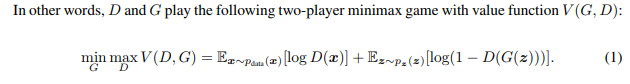
\includegraphics[width=\hsize]{./mokuteki.png}
	\end{center}
	\end{figure}
	\begin{figure}[htbp]
	\begin{center}
	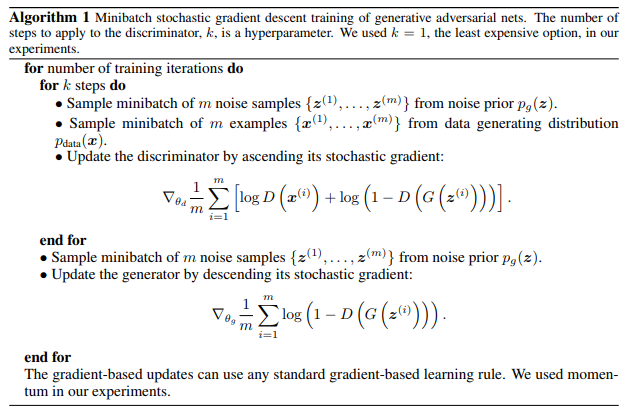
\includegraphics[width=\hsize]{./gaku.png}
	\end{center}
	\end{figure}
\end{frame}

\section{実装}
\subsection{学習}
\begin{frame}
	\frametitle{学習に3時間かかった}
	\begin{figure}[htbp]
	\begin{center}
	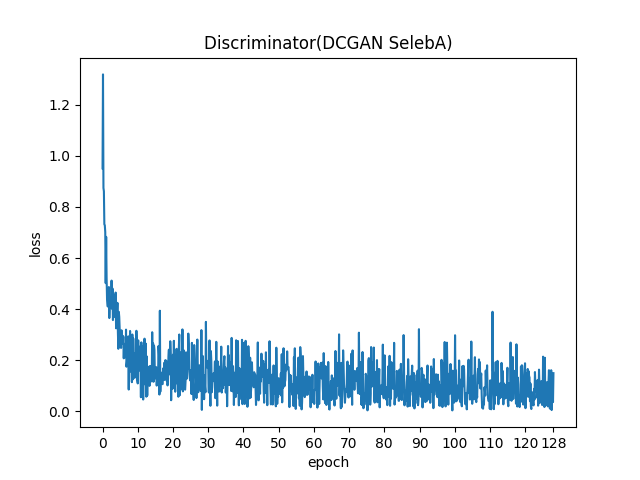
\includegraphics[width=0.5\hsize]{./dcgan_D.png}
	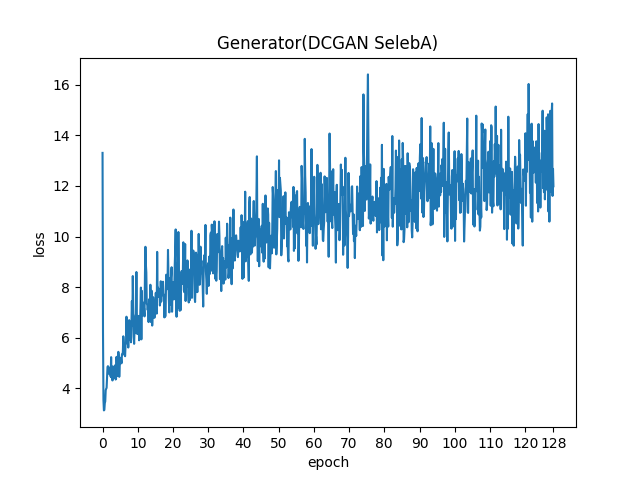
\includegraphics[width=0.5\hsize]{./dcgan_G.png}
	\end{center}
	\end{figure}
	dcgan inseption score : 1.5774693
\end{frame}
\subsection{生成画像}
%{{{
\begin{frame}
	\frametitle{10\%}
	\begin{figure}[htbp]
	\begin{center}
	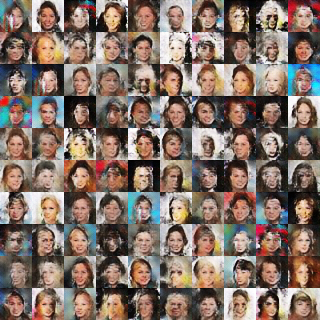
\includegraphics[width=0.7\hsize]{./dcgan/image00010000.png}
	\end{center}
	\end{figure}
\end{frame}
\begin{frame}
	\frametitle{20\%}
	\begin{figure}[htbp]
	\begin{center}
	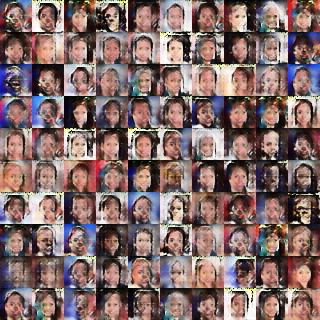
\includegraphics[width=0.7\hsize]{./dcgan/image00020000.png}
	\end{center}
	\end{figure}
\end{frame}
\begin{frame}
	\frametitle{30\%}
	\begin{figure}[htbp]
	\begin{center}
	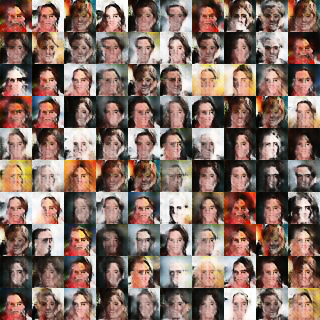
\includegraphics[width=0.7\hsize]{./dcgan/image00030000.png}
	\end{center}
	\end{figure}
\end{frame}
\begin{frame}
	\frametitle{40\%}
	\begin{figure}[htbp]
	\begin{center}
	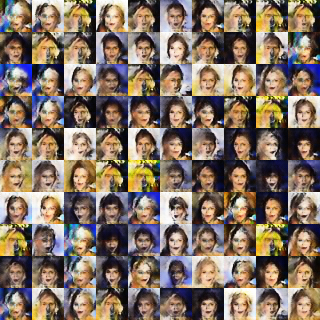
\includegraphics[width=0.7\hsize]{./dcgan/image00040000.png}
	\end{center}
	\end{figure}
\end{frame}
\begin{frame}
	\frametitle{50\%}
	\begin{figure}[htbp]
	\begin{center}
	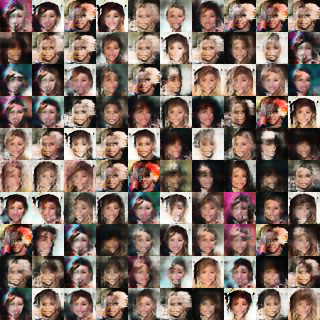
\includegraphics[width=0.7\hsize]{./dcgan/image00050000.png}
	\end{center}
	\end{figure}
\end{frame}
\begin{frame}
	\frametitle{60\%}
	\begin{figure}[htbp]
	\begin{center}
	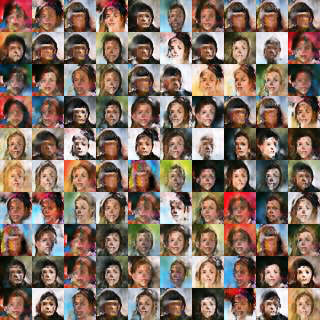
\includegraphics[width=0.7\hsize]{./dcgan/image00060000.png}
	\end{center}
	\end{figure}
\end{frame}
\begin{frame}
	\frametitle{70\%}
	\begin{figure}[htbp]
	\begin{center}
	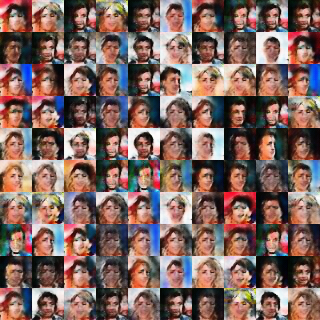
\includegraphics[width=0.7\hsize]{./dcgan/image00070000.png}
	\end{center}
	\end{figure}
\end{frame}
\begin{frame}
	\frametitle{80\%}
	\begin{figure}[htbp]
	\begin{center}
	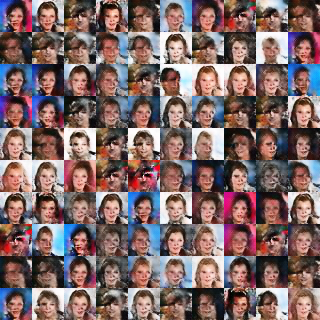
\includegraphics[width=0.7\hsize]{./dcgan/image00080000.png}
	\end{center}
	\end{figure}
\end{frame}
\begin{frame}
	\frametitle{90\%}
	\begin{figure}[htbp]
	\begin{center}
	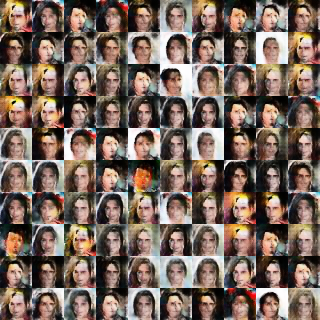
\includegraphics[width=0.7\hsize]{./dcgan/image00090000.png}
	\end{center}
	\end{figure}
\end{frame}
\begin{frame}
	\frametitle{100\%}
	\begin{figure}[htbp]
	\begin{center}
	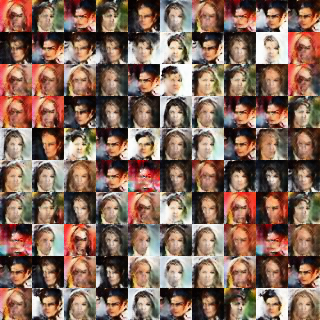
\includegraphics[width=0.7\hsize]{./dcgan/image00100000.png}
	\end{center}
	\end{figure}
\end{frame}
%}}}

\section{改善}
\subsection{spectral normalization}
\begin{frame}
	\frametitle{spectral normalization}
	\begin{figure}[htbp]
	\begin{center}
	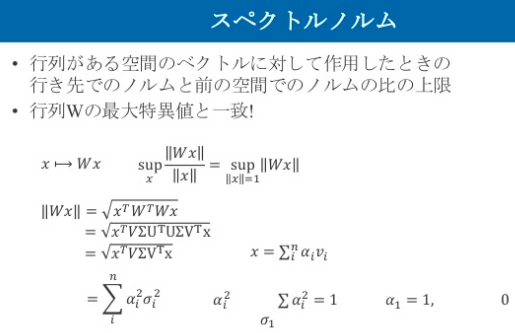
\includegraphics[width=\hsize]{./spec_dis.png}
	\end{center}
	\end{figure}
\end{frame}

\subsection{学習}
\begin{frame}
	\frametitle{学習に4時間かかった}
	\begin{figure}[htbp]
	\begin{center}
	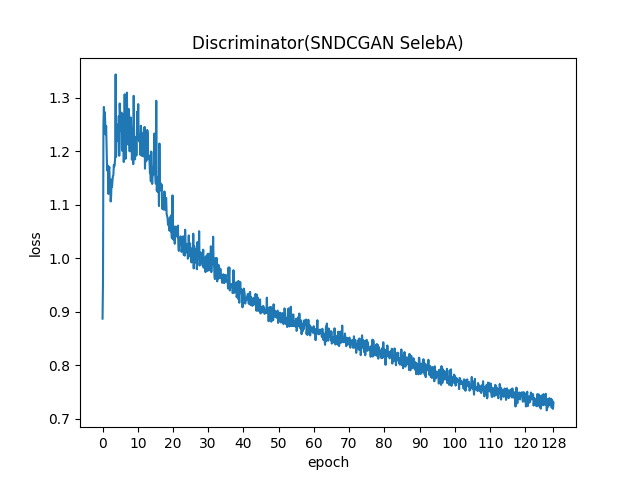
\includegraphics[width=0.5\hsize]{./sndcgan_D.png}
	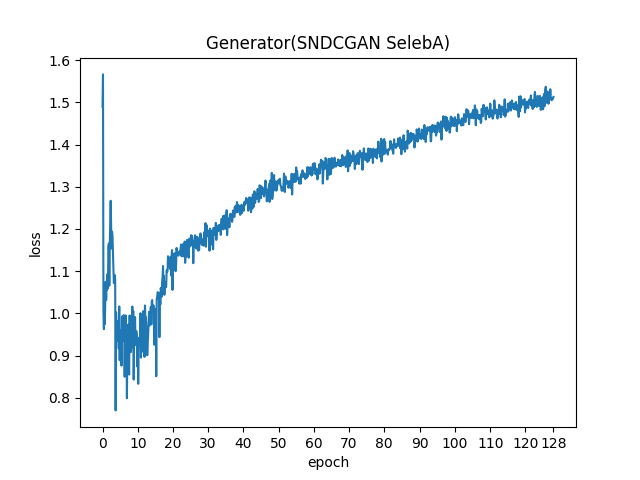
\includegraphics[width=0.5\hsize]{./sndcgan_G.png}
	\end{center}
	\end{figure}
	sndcgan inseption score : 1.5909373
\end{frame}

\subsection{生成画像}
%{{{
\begin{frame}
	\frametitle{10\%}
	\begin{figure}[htbp]
	\begin{center}
	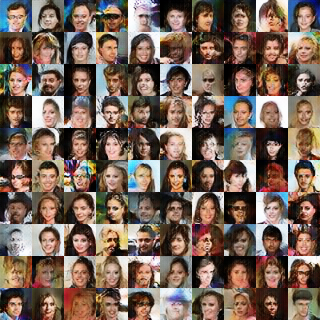
\includegraphics[width=0.7\hsize]{./sndcgan/image00010000.png}
	\end{center}
	\end{figure}
\end{frame}
\begin{frame}
	\frametitle{20\%}
	\begin{figure}[htbp]
	\begin{center}
	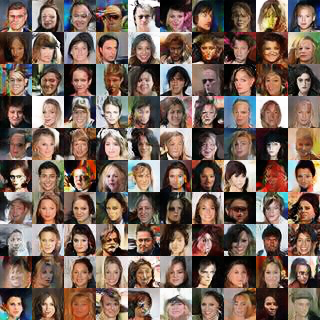
\includegraphics[width=0.7\hsize]{./sndcgan/image00020000.png}
	\end{center}
	\end{figure}
\end{frame}
\begin{frame}
	\frametitle{30\%}
	\begin{figure}[htbp]
	\begin{center}
	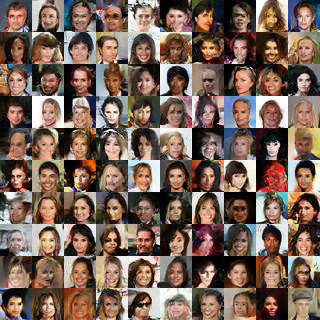
\includegraphics[width=0.7\hsize]{./sndcgan/image00030000.png}
	\end{center}
	\end{figure}
\end{frame}
\begin{frame}
	\frametitle{40\%}
	\begin{figure}[htbp]
	\begin{center}
	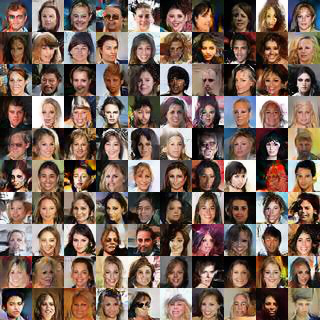
\includegraphics[width=0.7\hsize]{./sndcgan/image00040000.png}
	\end{center}
	\end{figure}
\end{frame}
\begin{frame}
	\frametitle{50\%}
	\begin{figure}[htbp]
	\begin{center}
	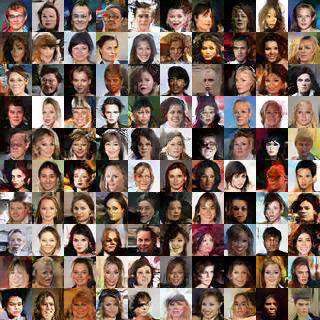
\includegraphics[width=0.7\hsize]{./sndcgan/image00050000.png}
	\end{center}
	\end{figure}
\end{frame}
\begin{frame}
	\frametitle{60\%}
	\begin{figure}[htbp]
	\begin{center}
	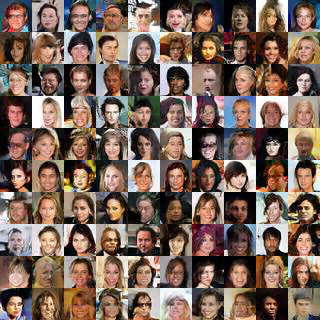
\includegraphics[width=0.7\hsize]{./sndcgan/image00060000.png}
	\end{center}
	\end{figure}
\end{frame}
\begin{frame}
	\frametitle{70\%}
	\begin{figure}[htbp]
	\begin{center}
	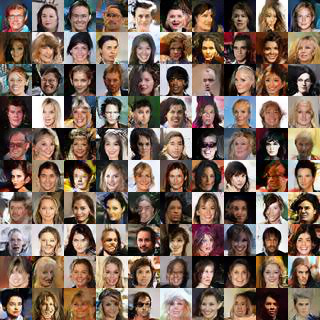
\includegraphics[width=0.7\hsize]{./sndcgan/image00070000.png}
	\end{center}
	\end{figure}
\end{frame}
\begin{frame}
	\frametitle{80\%}
	\begin{figure}[htbp]
	\begin{center}
	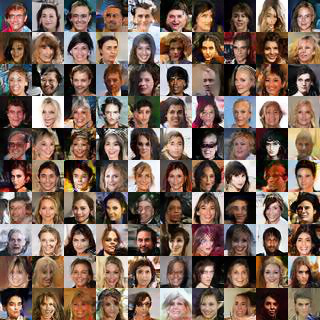
\includegraphics[width=0.7\hsize]{./sndcgan/image00080000.png}
	\end{center}
	\end{figure}
\end{frame}
\begin{frame}
	\frametitle{90\%}
	\begin{figure}[htbp]
	\begin{center}
	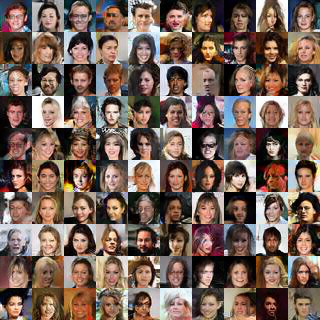
\includegraphics[width=0.7\hsize]{./sndcgan/image00090000.png}
	\end{center}
	\end{figure}
\end{frame}
\begin{frame}
	\frametitle{100\%}
	\begin{figure}[htbp]
	\begin{center}
	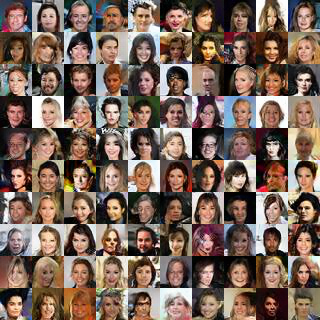
\includegraphics[width=0.7\hsize]{./sndcgan/image00100000.png}
	\end{center}
	\end{figure}
\end{frame}
%}}}

\section{結論}
\begin{frame}
	\frametitle{結論}
	spectral normalizationでinception scoreを上げることに成功した。\\
	学習が安定し、画像の多様性も増したように見える。\\
	github:
	\textcolor{blue}{
	\underline{
	\href{https://github.com/nat-chan/my-chainer-gan}{nat-chan/my-chainer-gan}
}}
	\href{https://github.com/nat-chan/HumanSensing}{nat-chan/HumanSensing}
	参考文献
%	\begin{thebibliography{9}
%		\bibitem{gan} Generative Adversarial Networks \url{https://arxiv.org/abs/1406.2661}
%		\bibitem{dcgan} 文献情報
%	\end{thebibliography}
\end{frame}
\end{document}
